\documentclass[12pt, a4paper, titlepage]{article}

\usepackage[spanish]{babel}
\usepackage[utf8]{inputenc}
\usepackage{graphicx}

% Margin set to a4wide
\usepackage{geometry}
\usepackage{layout}

\geometry{
  left=2.5cm,
  right=2.5cm,
  top=3.5cm,
  bottom=3cm
}

\usepackage{listings}
\usepackage{dirtree}
\usepackage{chicago}
\usepackage{multicol}
\usepackage{hyperref}

\linespread{1.3}

\title{
  \large{Diseño e Implementación de Compiladores}\\
  \huge{Diseño de un compilador para \textsc{compi}}
}

\author{
  Cardellino, Cristian $\cdot$ Leberle, Maico $\cdot$ Soldevila, Mallku
}

\date{31 de Octubre de 2015}

\begin{document}
  \maketitle

  \section{Introducción}

  Se presenta a continuación el informe del proyecto final de la materia
  ``Diseño e implementación de compiladores'', dictada como materia optativa y
  de posgrado en la carrera de Licenciatura en Ciencias de la Computación de la
  Facultad de Matemática, Astronomía y Física, en la Universidad Nacional de
  Córdoba.

  El objetivo de este proyecto es el diseño e implementación de un compilador
  para un lenguaje de programación imperativo simple, de estilo similar a C o
  Pascal, denominado \textsc{compi}.

  En el presente informe se reportan las caraterísticas del proyecto, los pasos
  seguidos en el desarrollo del mismo, y las desiciones de diseño tomadas
  durante las etapas, entre otros temas de distinta índole respecto al panorama
  general del proyecto.

  El siguiente documento se organiza de la siguiente manera: la sección
  \ref{sec:struct} describe la estructura del directorio del proyecto y explica
  como compilarlo y correr la suite de tests del mismo.

  \section{Estructura del Proyecto}\label{sec:struct}

  El proyecto se encuentra disponible libremente en el repositorio
  \url{https://github.com/MaicoLeberle/COMPIcompiler}. La estructura de
  directorios es la siguiente:

  \dirtree{%
    .1 ./compi.
    .2 bin.
    .2 build.
    .2 doc.
    .3 design\_decisions.
    .3 report.
    .2 src.
    .3 parser.
    .3 tests.
    .2 test.
  }

  En el directorio raíz ({\tt compi}) se encuentra el {\tt Makefile} para
  compilar el ejecutable de {\tt compi} y crear un ejecutable para correr una
  suite de tests. Por defecto, correr {\tt make}, crea compi y la suite de
  tests.

  El directorio {\tt bin} es el destino del ejecutable de {\sc compi} una vez
  finalizado todo el proceso de compilación y enlace del mismo. Además, también
  es el destino de la suite de tests.

  El directorio {\tt build} es el destino de todos los archivos compilados
  intermedios (es decir, sin enlace), además del destino de los archivos fuente
  generados automáticamente por Flex y Bison.

  El directorio {\tt doc} tiene dos subdirectorios: {\tt design\_decisions}
  contiene algunas notas sobre las decisiones de diseño que se tomaron a lo
  largo del proyecto, como el diseño del {\em Abstract Syntax Tree} (AST),
  decisiones sobre como trabajar con las llamadas {\em locations} (i.e. las
  referencias a un atributo de algún objeto) o decisiones respecto al {\em
  scope}; por otro lado, el directorio {\tt report}, contiene el código fuente
  latex de este informe.

  El directorio {\tt src} contiene el código fuente de {\sc compi}. En el
  subdirectorio {\tt parser}, está el código fuente de Flex y Bison, que vienen
  a representar la tokenización y gramática del lenguaje compi, a su vez, dentro
  de este subdirectorio existen otros dos: {\tt parser\_asm}, que contiene la
  tokenización y gramática del código assembly; y {\tt parser\_ir} que contiene
  la tokenización y gramática del código intermedio.

  Por otra parte, también dentro de {\tt src}, pero en el subdirectorio {\tt
  tests}, se encuentra el código fuente de la suite de tests para {\sc compi}.

  Finalmente, en el directorio {\tt test}, se encuentra una serie de archivos en
  código {\sc compi} que son utilizados para los tests.

  Como se mencionó previamente, corriendo {\tt make}, se genera el ejecutable de
  {\sc compi} así como también la suite de tests. El ejecutable del compilador
  se encuentra en {\tt ./bin/compi}, la suite de tests se encuentra en {\tt
  ./bin/test}. Al correr la suite de tests a través del ejecutable
  correspondiente, corre todos los tests que se escribieron para la aplicación.

  \section{Arquitectura del Proyecto}\label{sec:architecture}

  La arquitectura puede observarse en la Figura \ref{fig:architecture}. Se
  muestra aquí el flujo de operaciones desde el código fuente de COMPI hasta la
  obtención del código Assembly que lo representa.

  \begin{figure}[h]
    \centering
    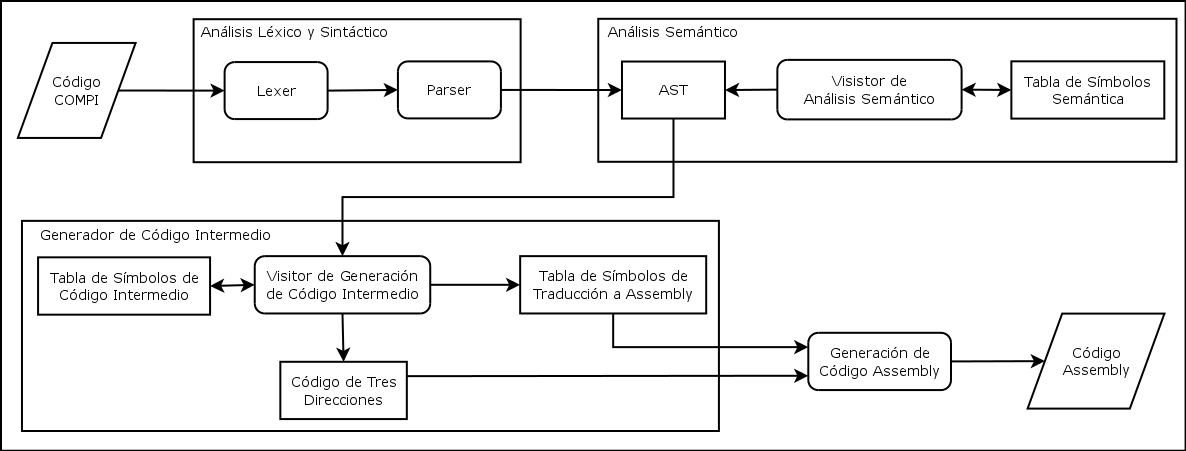
\includegraphics[width=\textwidth]{architecture.png}
    \caption{Arquitectura de COMPI}
    \label{fig:architecture}
  \end{figure}

  A partir del código fuente en COMPI, el primer paso se da a través del {\bf
  análisis léxico y sintáctico}. El lexer determina los tokens a procesar,
  identificando palabras reservadas, literales, etc. Esto se hace mediante la
  herramienta {\tt flex}. Se sigue del parser, que toma los elementos devueltos
  por el lexer y, siguiendo la gramática definida para el lenguaje, crea los
  nodos del árbol sintáctico. La herramienta que se encarga de parsear es {\tt
  bison}.

  Una vez terminada la etapa de análisis léxico y sintáctico, se sigue la etapa
  de {\bf análisis semántico}. La etapa arranca a partir del {\em abstract
  syntax tree} (AST o árbol sintáctico abstracto), que fue generado en la etapa
  anterior por el parser. Sobre el AST obtenido se aplica un {\em patrón
  visitor}, que crea y utiliza una tabla de símbolos localmente para comprobar
  distintos elementos de la semántica del lenguaje: tipos y alcance/visibilidad
  de los identificadores, asignaciones, número de parámetros y valor de retorno
  en las funciones, etc. Además de revisar con detenimiento ciertas reglas
  semánticas, como la declaración de identificadores y su llamada, la existencia
  de un método {\em main}, la correcta declaración de arreglos, entre otras
  restricciones definidas en las descripciones del lenguaje.

  Concluída la verificación semántica del AST pasamos a la etapa de {\bf
  generación de código intermedio}. El AST es recorrido nuevamente por un {\em
  patrón visitor}, que en este punto busca generar el código intermedio,
  definido como un código de tres direcciones. A través de una tabla de símbolos
  interna al proceso, se guarda información del alcance de los identificadores,
  así como cualquier otra información necesaria para luego generar el código
  intermedio de tres direcciones (e.g., tipo de la variable, el offset dentro
  del cuerpo del método, las variable, etc.). Este proceso genera dos recursos:
  el código de tres direcciones, que viene a ser el código intermedio de la
  aplicación y la tabla de traducción de símbolos para la traducción a Assembly,
  que guarda directamente información sobre las variables a utilizar en el
  código assembly.

  A partir de los recursos generados en la parte anterior se entra en la etapa
  de {\bf generación de código assembly}, que producirá un archivo en código
  assembly que luego será compilado mediante el compilador correspondiente.

  \section{Decisiones de Diseño}\label{sec:design}

  Para la creación del AST nos basamos en la estructura propuesta en la serie de
  posts de la página {\em gnuu}, llamado ``Writing Your Own Toy Compiler Using
  Flex, Bison and LLVM''
  \footnote{\url{http://gnuu.org/2009/09/18/writing-your-own-toy-compiler/}}.
  Este fue adaptado a los requerimientos del lenguaje COMPI. Todos los nodos
  heredan de una clase principal {\em node} que a grandes razgos se diferencia
  entre declaraciones (de métodos y variables), órdenes de flujo ({\em
  statements}, en inglés) y expresiones (matemáticas, comparativas, lógicas).

  \section{Conclusiones}\label{sec:conclusions}
\end{document}

% La sección
% \ref{sec:spec} describe las características del lenguaje \textsc{compi}:
% léxico, gramática y semántica.
%
% Como se modulariza, como se compila y como se pueden correr los ejemplos y
% {\em tests}.

% \section{Especificaciones de COMPI}\label{sec:spec}
%
% Un programa {\sc compi} consiste en una lista de declaraciones de clases,
% atributos y métodos. Estos atributos son variables globales que pueden ser
% accedidas por todos los métodos de la clase y por todos los objetos
% instanciados de una clase. Los objetos referencian sus atributos e invocan sus
% métodos con la notacin habitual. Ambos, atributos y mtodos son siempre
% públicos ya que el lenguaje no tiene modificadores de visibilidad. El lenguaje
% no permite la creación dinámica de objetos.
%
% La declaración de métodos define funciones y procedimientos. El programa debe
% contener la declaración de una clase llamada {\bf main} con un método llamado
% del mismo nombre. Este método no tiene parámetros. La ejecución de un programa
% COMPI comienza con el método {\bf main}.
%
% El lenguaje {\sc compi} es case-sensitive. De igual manera, lo son las
% palabras reservadas y los identificadores del mismo.
%
% La palabras reservadas son las siguientes:
% \begin{multicols}{5}
%   \begin{itemize}
%     \item boolean
%     \item break
%     \item class
%     \item continue
%     \item else
%     \item false
%     \item float
%     \item for
%     \item if
%     \item int
%     \item return
%     \item true
%     \item void
%     \item while
%     \item extern
%   \end{itemize}
% \end{multicols}
%
% El lenguaje acepta comentarios, de una sola línea con {\bf //} o de múltiples
% líneas, delimitado por {\bf /*} y {\bf */}. Los literales del lenguaje son
% cadenas de caracteres, enteros y reales.
%
% Los tipos básicos de {\sc compi} son {\bf int}, {\bf float} y {\bf boolean}.
%
% Un ejemplo de programa en {\sc compi} es:
%
% \begin{verbatim}
%   class Program {
%     int inc(int x) {
%       return x + 1;
%     }
%     int read_int() extern;
%     void print(string s) extern;
%     void main() {
%       int y;
%       y = read_int();
%       y = inc(y);
%       if (y == 1)
%         printf("y==1\n");
%       else
%         printf("y!=1\n");
%     }
%   }
% \end{verbatim}
